\documentclass[../Article_Sensitivity_Analsysis.tex]{subfiles}
\graphicspath{{\subfix{../Figures/}}}
\begin{document}
	
	\label{CH: Results}
	
	%To identify the global solution of the Equation \ref{EQ:Formulation}, the optimization problem is solved multiple times starting from random initial solutions. The solution with the lowest value of the cost function is considered to be the global solution. Figure \ref{fig:scatter}, show an compression between initial and the final values of the cost function for multiple optimization problems. The shaded area is spanned between the smallest and the third smallest final value of the objective function. The black curves on the left and below of the scatter plot indicate distributions of the initial and final values of the cost function, respectively.
	
	To identify the global solution of Equation \ref{EQ:Formulation}, the optimization problem is solved multiple times starting from random initial solutions. The solution with the lowest cost function value is considered the global solution. Figure \ref{fig:scatter} shows a comparison between the initial and final values of the cost function for multiple optimization runs. The shaded area spans from the smallest to the third smallest final value of the objective function. The black curves on the left and below the scatter plot indicate the distributions of the initial and final cost function values, respectively.
	
	\begin{figure}[h!]
		\centering
		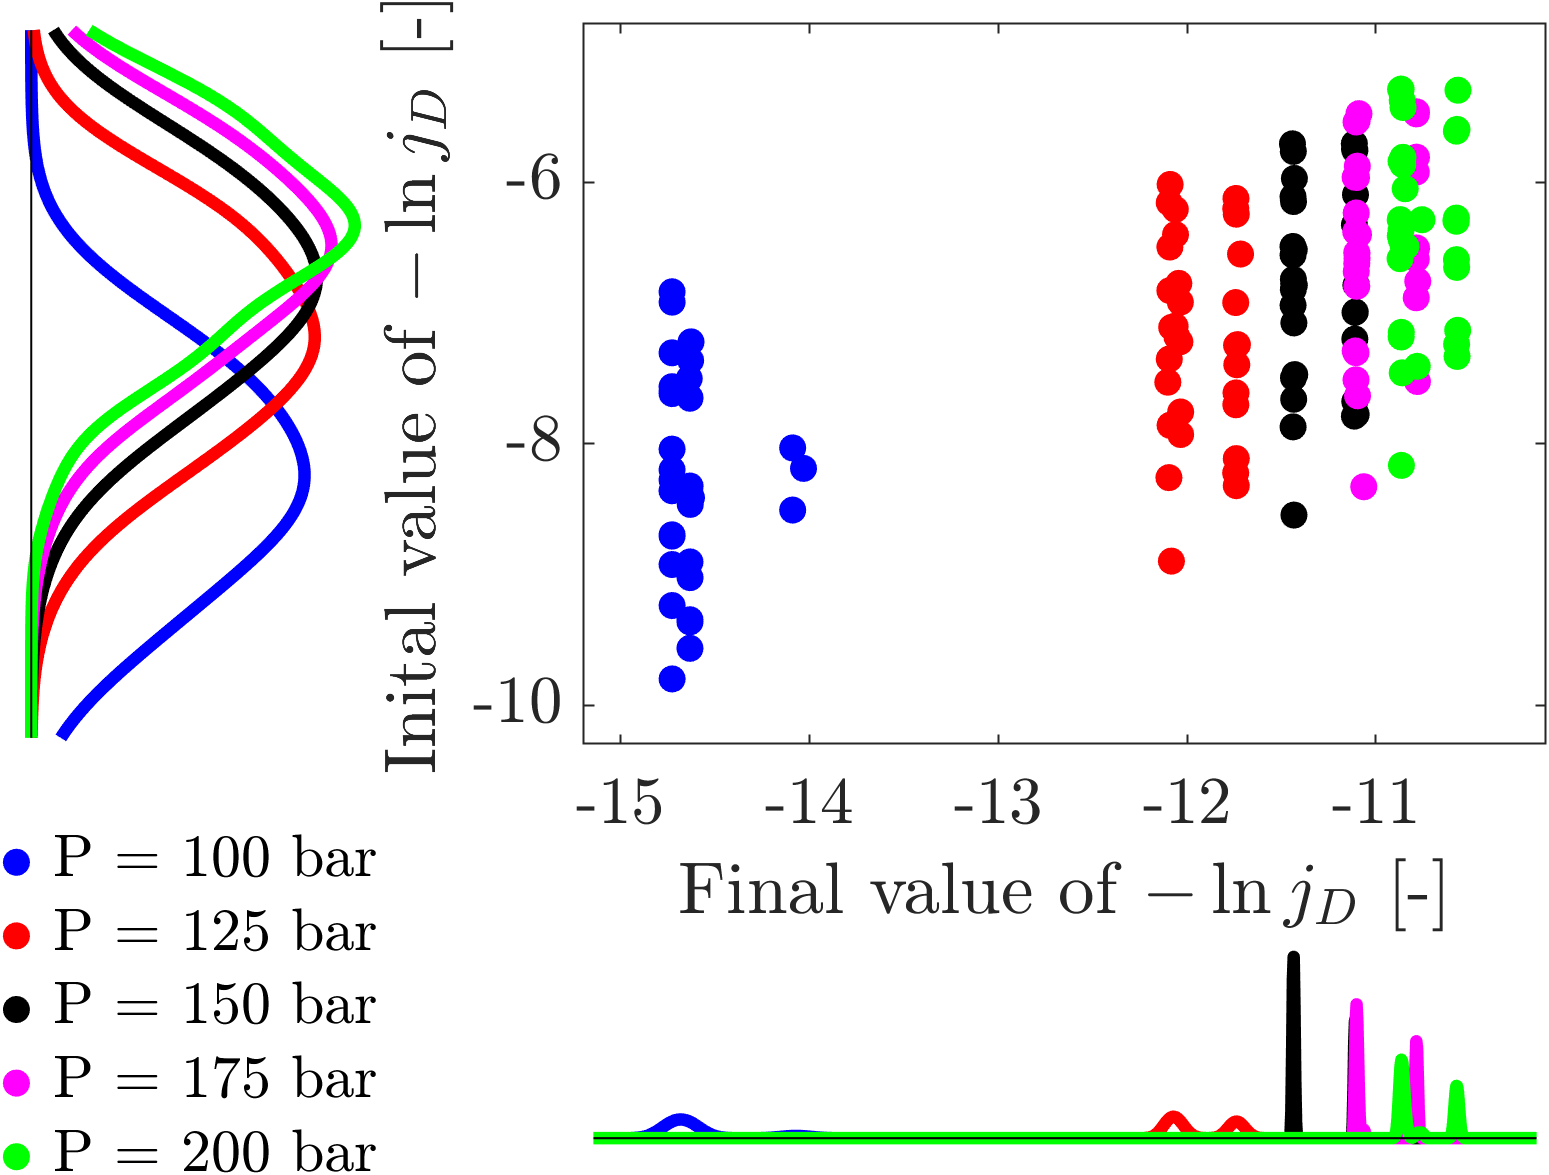
\includegraphics[width=\columnwidth]{Figures/Results/scatter.png}	
		\caption{Initial vs final values of the cost function}
		\label{fig:scatter}
	\end{figure}
	
	The optimal inlet temperature and mass flow rate profile are presented on Figure \ref{fig:profile}. 
	
	\begin{figure}[h!]
		\centering
		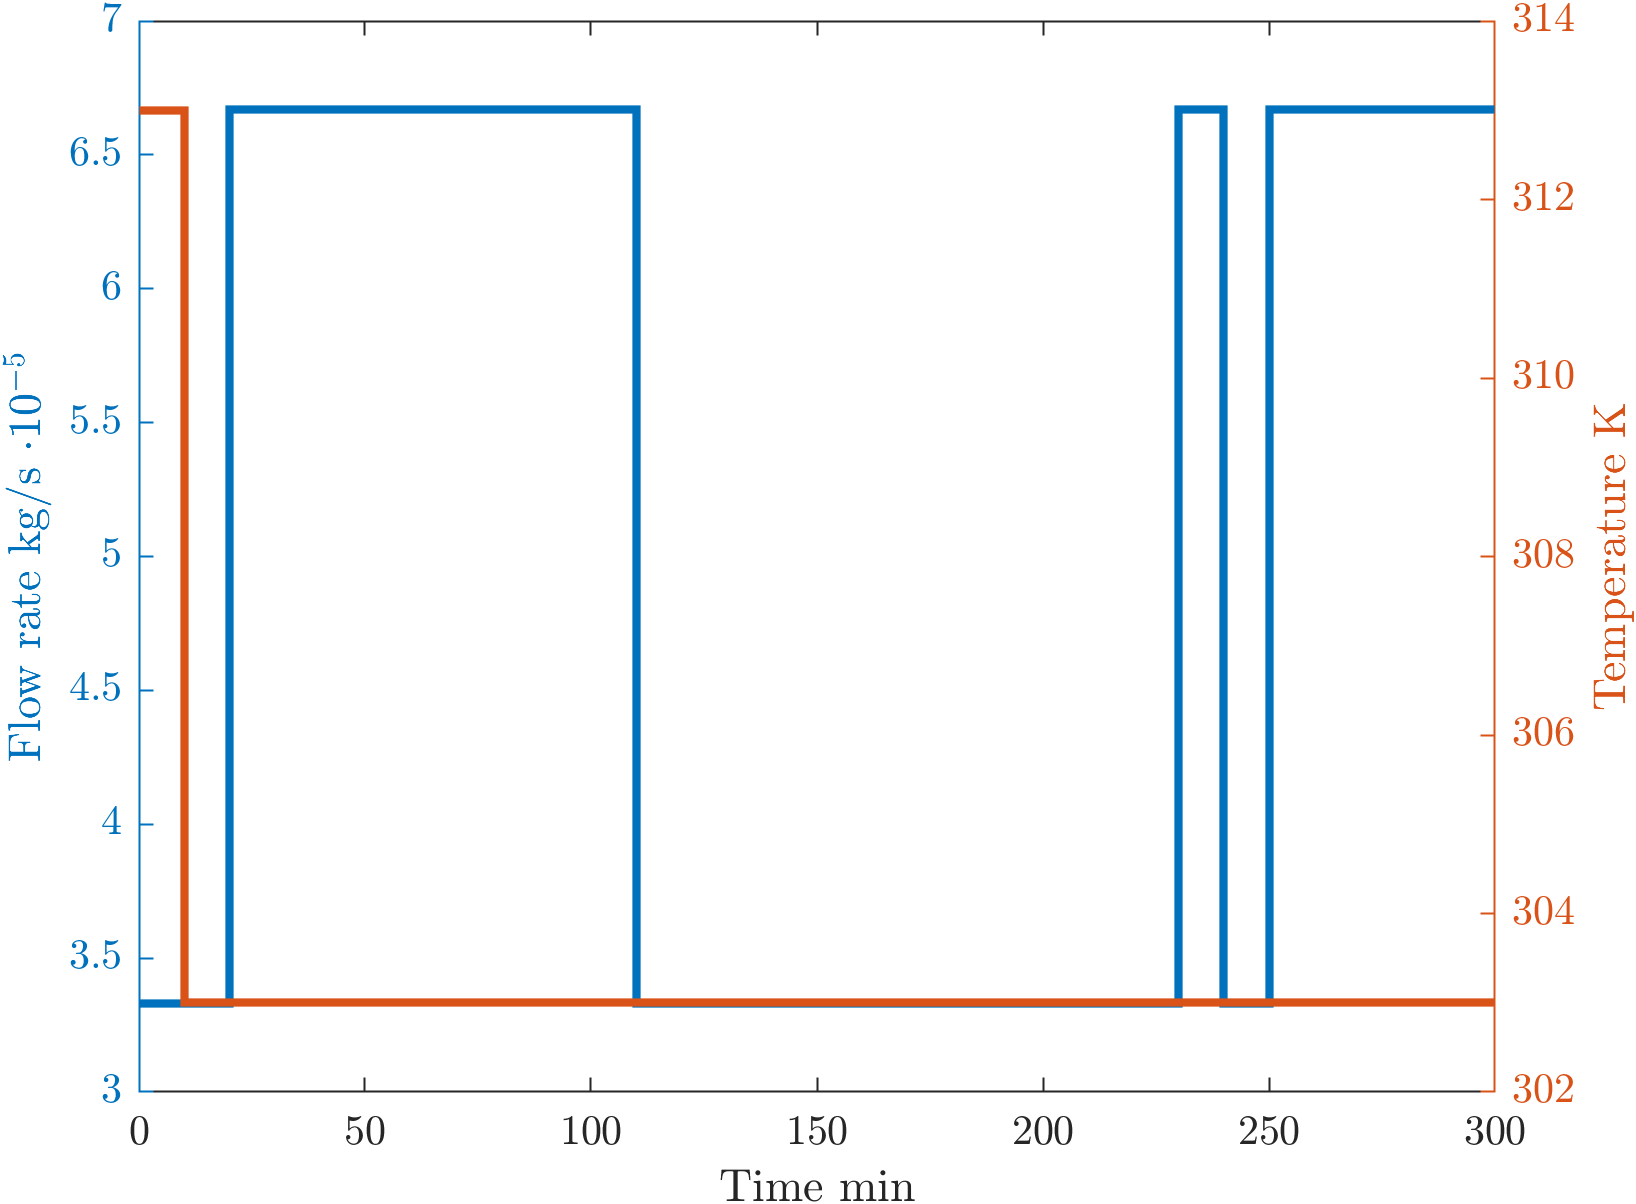
\includegraphics[width=\columnwidth]{Figures/Results/Profile.png}	
		\caption{Optimal temperature and mass flow rate profiles}
		\label{fig:profile}
	\end{figure}
	
	\begin{comment}
		\begin{figure}[h!]
			\centering
			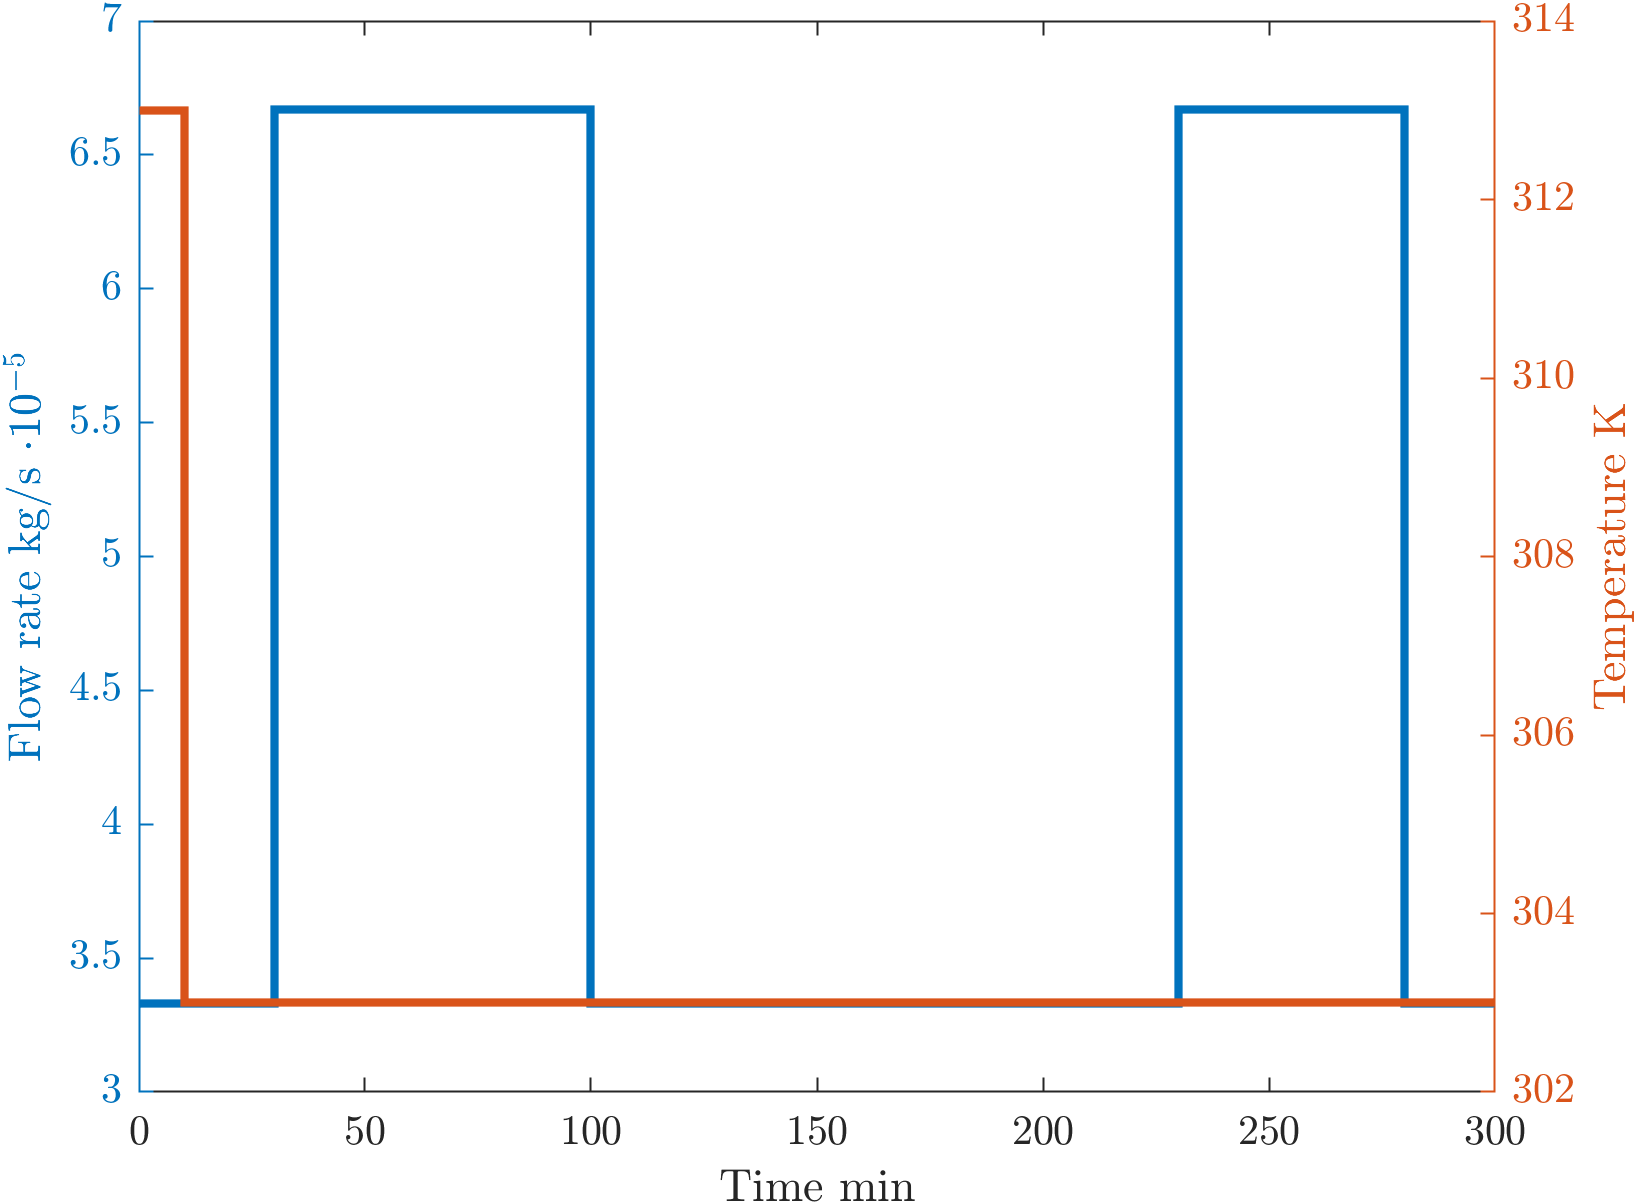
\includegraphics[width=\columnwidth]{Figures/Results/Profile_2.png}	
			\caption{2nd Optimal temperature and mass flow rate profiles}
			\label{fig:profile_2}
		\end{figure}
		
		\begin{figure}[h!]
			\centering
			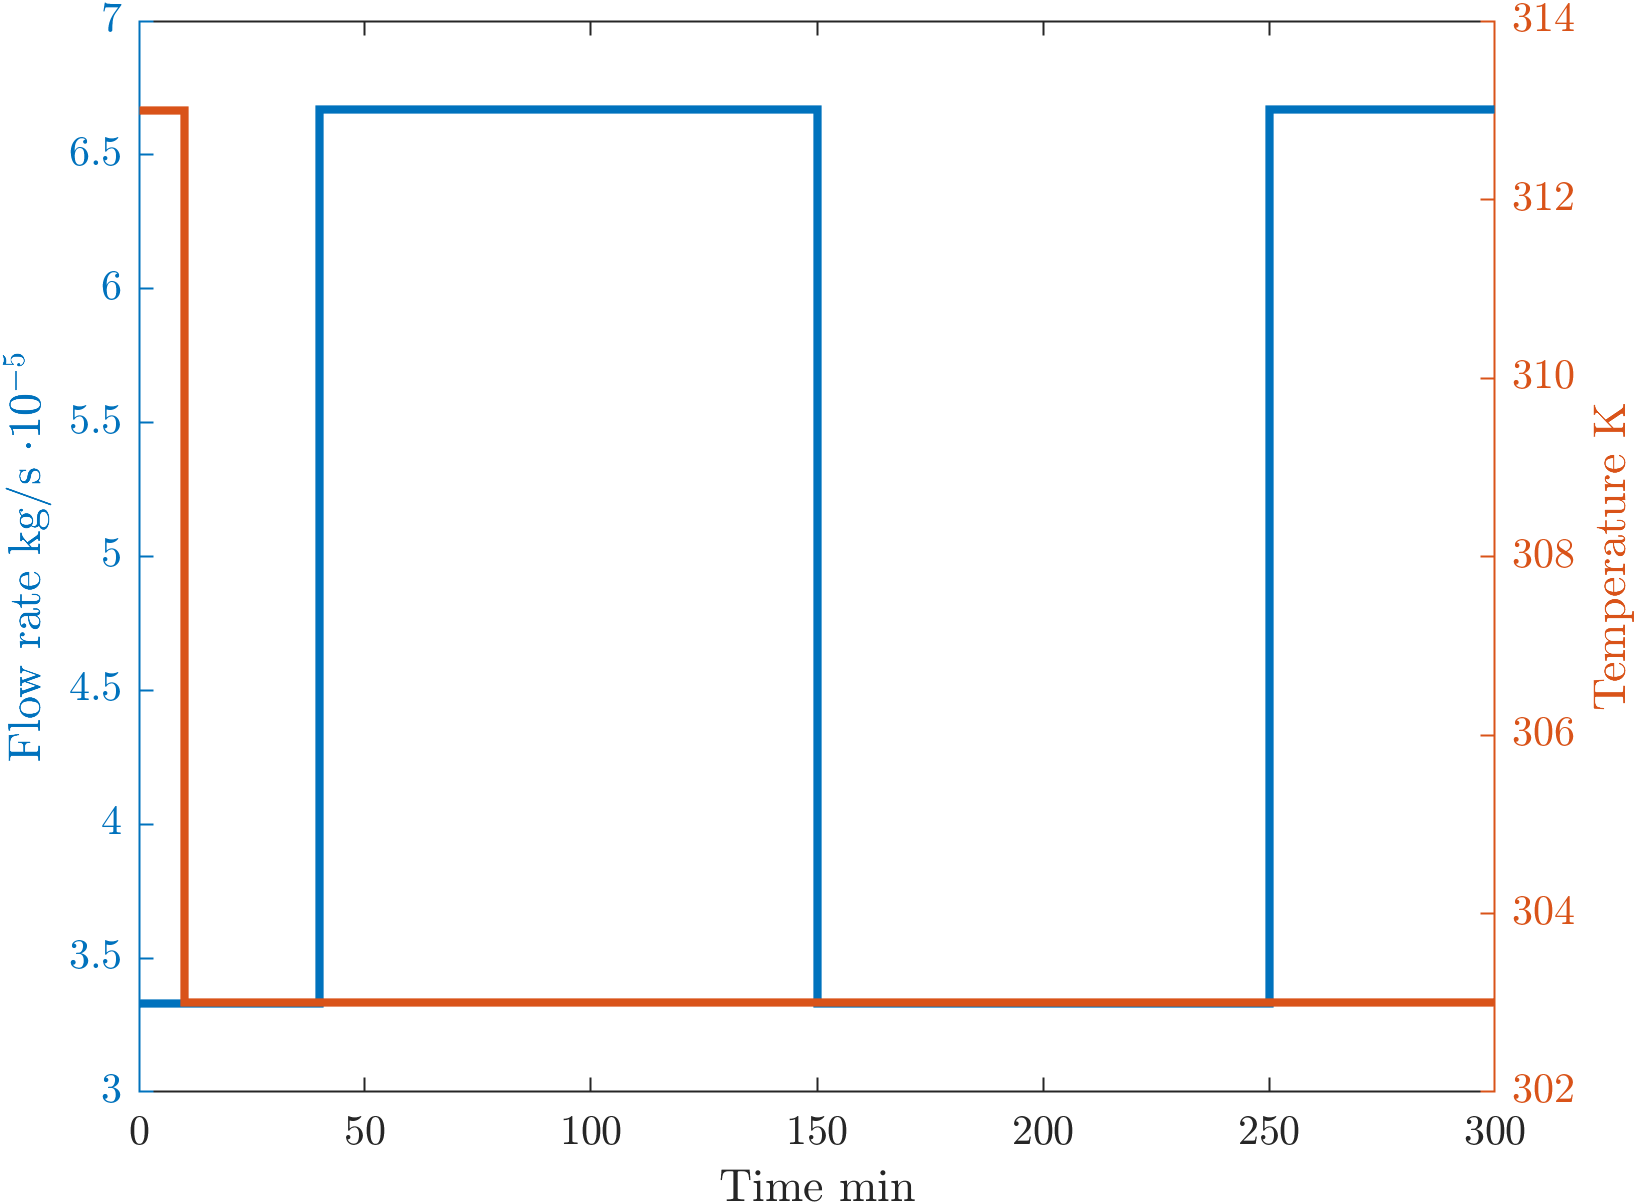
\includegraphics[width=\columnwidth]{Figures/Results/Profile_3.png}	
			\caption{3rd Optimal temperature and mass flow rate profiles}
			\label{fig:profile_3}
		\end{figure}
	\end{comment}
	
\end{document}